\documentclass{beamer}
\usetheme{Madrid}
\usecolortheme{whale}

\usepackage{graphicx}
\usepackage{tikz}
\usetikzlibrary{shapes.geometric, arrows.meta, positioning, calc}
\usepackage{booktabs}
\usepackage{listings}
\usepackage{algorithm}
\usepackage{algorithmic}
\usepackage{amsmath}
\usepackage{amssymb}
\usepackage{multirow}
\usepackage{array}

% Define Verilog listing style for presentation
\lstdefinelanguage{Verilog}{
  morekeywords={module, input, output, wire, reg, parameter, localparam, always, assign, begin, end, case, default, endcase, posedge, negedge, if, else, initial},
  sensitive=true,
  morecomment=[l]{//},
  morecomment=[s]{/*}{*/},
  morestring=[b]"
}

\lstset{
  language=Verilog,
  basicstyle=\ttfamily\tiny,
  keywordstyle=\color{blue}\bfseries,
  commentstyle=\color{gray},
  stringstyle=\color{purple},
  backgroundcolor=\color{white},
  showspaces=false,
  showstringspaces=false,
  showtabs=false,
  frame=single,
  tabsize=2,
  breaklines=true,
}

% Custom commands and metadata
\title[Scalable SPI Bus Interface]{Design and FPGA Implementation of a Scalable SPI Bus Interface Supporting Multiple Sensors with Variable Data Widths}
\author{Bhargav Vemparala}
\institute[Evaluation Board]{Department of Electrical and Computer Engineering \\ University Evaluation Board}
\date{July 20, 2026}

\begin{document}

% Slide 1: Title Slide
\begin{frame}
  \titlepage
\end{frame}

% Slide 2: Table of Contents
\begin{frame}{Presentation Outline}
  \tableofcontents
\end{frame}

\section{Introduction \& Evolution}

% Slide 3: Motivation
\begin{frame}{Introduction \& Motivation}
  \begin{itemize}
    \item \textbf{Problem with Traditional SPI:} 
    \begin{itemize}
      \item Standard SPI requires a dedicated Chip Select (CS) line for each slave.
      \item For $N$ devices, wiring complexity is $O(N)$ (requires $N+3$ wires).
      \item Consumes valuable GPIO pins on the host MCU and increases routing congestion.
    \end{itemize}
    \item \textbf{Proposed Solution:}
    \begin{itemize}
      \item Design an intelligent intermediary \textbf{SPI Bus Interface} on an FPGA.
      \item Share a single 3-wire/4-wire bus among all sensors.
      \item Virtualize sensor registers on-chip, reducing wiring complexity to $O(1)$.
    \end{itemize}
  \end{itemize}
\end{frame}

% Slide 4: Design Evolution
\begin{frame}{Design Evolution}
  \begin{columns}
    \begin{column}{0.5\textwidth}
      \textbf{Iteration 1: Proof-of-Concept}
      \begin{itemize}
        \item Single SPI slave, direct interface.
        \item Fixed 1-bit input/output width.
        \item Simple 5-state machine.
        \item High protocol overhead.
      \end{itemize}
      \vspace{0.2cm}
      \textbf{Iteration 2: Burst-Mode Interface}
      \begin{itemize}
        \item Introduces address decoding.
        \item Fixed 4-bit burst length.
        \item Inflexible for asymmetric sensors.
      \end{itemize}
    \end{column}
    \begin{column}{0.5\textwidth}
      \textbf{Iteration 3: Scalable Architecture (Final)}
      \begin{itemize}
        \item Supports heterogeneous sensors.
        \item Allows completely different input/output widths.
        \item Dynamic packet handling.
        \item Fully decoupled master/sensor communication.
      \end{itemize}
    \end{column}
  \end{columns}
\end{frame}

\section{System Architecture}

% Slide 5: System Architecture Diagram
\begin{frame}{System Block Diagram}
  \centering
  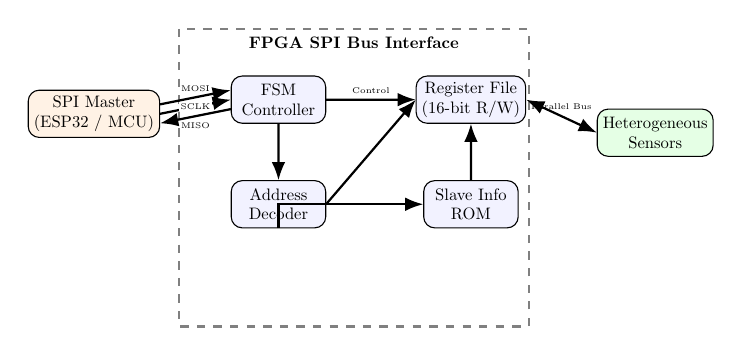
\begin{tikzpicture}[
      scale=0.6, every node/.style={transform shape},
      node distance=1.2cm and 1.5cm,
      block/.style={draw, rectangle, minimum height=1.0cm, minimum width=2.0cm, align=center, fill=blue!5, rounded corners},
      line/.style={draw, -{Latex[scale=1.0]}, thick},
      doubleline/.style={draw, {Latex[scale=1.0]}-{Latex[scale=1.0]}, thick}
  ]
      % Draw Master Block
      \node [block, fill=orange!10] (master) {SPI Master\\(ESP32 / MCU)};
      
      % Draw Bus Interface Boundary (FPGA)
      \draw[dashed, color=gray, thick] (1.8, 1.8) rectangle (9.2, -4.5);
      \node at (5.5, 1.5) {\textbf{FPGA SPI Bus Interface}};

      % Draw Internal Components
      \node [block, right=of master, yshift=0.3cm] (fsm) {FSM\\Controller};
      \node [block, below=of fsm] (decoder) {Address\\Decoder};
      \node [block, right=of fsm, xshift=0.4cm] (regs) {Register File\\(16-bit R/W)};
      \node [block, below=of regs] (rom) {Slave Info\\ROM};
      
      % Draw Sensors Block
      \node [block, right=of regs, fill=green!10, yshift=-0.7cm] (sensors) {Heterogeneous\\Sensors};
      
      % Connect Master to Interface
      \path [line] ($(master.east)+(0,0.2)$) -- node[above, font=\tiny] {MOSI} ($(fsm.west)+(0,0.2)$);
      \path [line] ($(fsm.west)+(0,-0.2)$) -- node[below, font=\tiny] {MISO} ($(master.east)+(0,-0.2)$);
      \path [line] (master.east) -- node[fill=white, inner sep=1pt, font=\tiny] {SCLK} (fsm.west);
      
      % Connect internal modules
      \path [line] (fsm.south) -- (decoder.north);
      \path [line] (decoder.east) -- (regs.west);
      \path [line] (decoder.south) |- (rom.west);
      \path [line] (rom.north) -- (regs.south);
      \path [line] (fsm.east) -- node[above, font=\tiny] {Control} (regs.west);
      
      % Connect Interface to Sensors
      \path [doubleline] (regs.east) -- node[above, font=\tiny] {Parallel Bus} (sensors.west);
  \end{tikzpicture}
\end{frame}

% Slide 6: Clock Domain Crossing (CDC)
\begin{frame}{Clock Domain Crossing \& FIFO Synchronization}
  \begin{itemize}
    \item \textbf{Asynchronous domains:} Sensors sample on $\text{CLK}_{\text{sensor}}$ while the host communicates on asynchronous $\text{SCLK}$.
    \item \textbf{Metastability Prevention:} 
    \begin{itemize}
      \item Directly sampling cross-domain registers can lead to timing violations and system failure.
      \item Integrated an \textbf{Asynchronous CDC FIFO} block (16-bit width, depth 8) between domains.
      \item Write port is driven by $\text{CLK}_{\text{sensor}}$ (valid flag controls writes).
      \item Read port is driven by $\text{SCLK}$ (controller pops values synchronously).
      \item Gray code counter logic guarantees safe pointer crossings.
    \end{itemize}
  \end{itemize}
\end{frame}

\section{Implemented Methodologies}

% Slide 7: Method 1: Address + Length
\begin{frame}{Method 1: Address + Bit-Length Protocol}
  \begin{itemize}
    \item \textbf{Dynamic Packet Concept:} 
    \begin{itemize}
      \item Master controls the exact size of write transactions on the fly.
      \item Sends \textbf{Mode (2 bits)}, \textbf{Address (5 bits)}, and \textbf{Length (4 bits)}, followed by data.
      \item Reads are \textbf{Master-Terminated}: Master holds MOSI high to receive consecutive bits, pulls MOSI low to stop.
    \end{itemize}
    \item \textbf{Packet Formats:}
    \begin{table}
      \centering\tiny
      \begin{tabular}{lcccc}
        \toprule
        \textbf{Op} & \textbf{Mode (2b)} & \textbf{Address (5b)} & \textbf{Length (4b)} & \textbf{Data Payload} \\
        \midrule
        Read & \texttt{00} & $A_4 \dots A_0$ & N/A & Dynamic (MoSi=0 to stop) \\
        Write & \texttt{01} & $A_4 \dots A_0$ & $L_3 \dots L_0$ & Variable ($L+1$ bits) \\
        \bottomrule
      \end{tabular}
    \end{table}
    \item \textbf{Pros \& Cons:} 
    \begin{itemize}
      \item \textit{Advantage:} Highly flexible. Widths are software-defined.
      \item \textit{Disadvantage:} High transaction overhead (11 bits of control for every write).
    \end{itemize}
  \end{itemize}
\end{frame}

% Slide 8: Method 1 FSM
\begin{frame}{Method 1: State Machine Diagram}
  \centering
  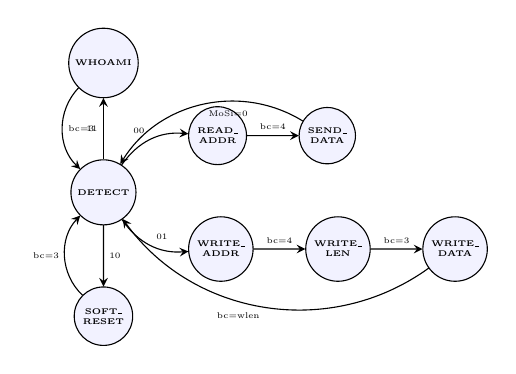
\begin{tikzpicture}[
      scale=0.6, every node/.style={transform shape},
      ->, >=stealth, node distance=1.3cm and 1.1cm,
      state/.style={circle, draw, minimum size=1.0cm, font=\tiny\bfseries, align=center, fill=blue!5},
      transition/.style={font=\tiny, auto}
  ]
      \node[state] (detect) {DETECT};
      \node[state, right=of detect, yshift=1.2cm] (raddr) {READ\_\\ADDR};
      \node[state, right=of raddr] (rdata) {SEND\_\\DATA};
      \node[state, right=of detect, yshift=-1.2cm] (waddr) {WRITE\_\\ADDR};
      \node[state, right=of waddr] (wlen) {WRITE\_\\LEN};
      \node[state, right=of wlen] (wdata) {WRITE\_\\DATA};
      \node[state, below=of detect] (srst) {SOFT\_\\RESET};
      \node[state, above=of detect] (who) {WHOAMI};

      \path (detect) edge[bend left] node[transition] {00} (raddr);
      \path (detect) edge[bend right] node[transition] {01} (waddr);
      \path (detect) edge node[transition] {10} (srst);
      \path (detect) edge node[transition] {11} (who);
      
      \path (raddr) edge node[transition] {bc=4} (rdata);
      \path (rdata) edge[bend right=45] node[transition] {MoSi=0} (detect);
      
      \path (waddr) edge node[transition] {bc=4} (wlen);
      \path (wlen) edge node[transition] {bc=3} (wdata);
      \path (wdata) edge[bend left=45] node[transition] {bc=wlen} (detect);
      
      \path (srst) edge[bend left=45] node[transition] {bc=3} (detect);
      \path (who) edge[bend right=45] node[transition] {bc=3} (detect);
  \end{tikzpicture}
\end{frame}

% Slide 9: Method 1 Write Algorithm
\begin{frame}[fragile]{Method 1: Master Write Algorithm}
  \begin{block}{Master Write Operation}
    \begin{algorithmic}[1]
      \STATE Assert $\text{CS} \leftarrow 0$
      \STATE Shift out \texttt{Mode = 01} (Write)
      \STATE Shift out 5-bit register address $A$
      \STATE Shift out 4-bit write length $L$
      \FOR{$i = 0$ \TO $L$}
        \STATE Shift out payload bit on MOSI
        \STATE Controller writes $\text{write\_reg}[(A + i) \pmod{16}] \leftarrow \text{MOSI}$
      \ENDFOR
      \STATE Deassert $\text{CS} \leftarrow 1$
    \end{algorithmic}
  \end{block}
\end{frame}

% Slide 10: Method 1 Read Algorithm
\begin{frame}[fragile]{Method 1: Master Read Algorithm}
  \begin{block}{Master Read Operation}
    \begin{algorithmic}[1]
      \STATE Assert $\text{CS} \leftarrow 0$
      \STATE Shift out \texttt{Mode = 00} (Read), 5-bit address $A$
      \STATE Initialize $i \leftarrow 0$
      \WHILE{MOSI is driven high (\texttt{1}) by Master}
        \STATE Read MISO bit $\leftarrow \text{read\_reg}[(A + i) \pmod{16}]$
        \STATE Increment $i \leftarrow i + 1$
      \ENDWHILE
      \STATE Deassert $\text{CS} \leftarrow 1$
    \end{algorithmic}
  \end{block}
\end{frame}

% Slide 9: Method 2: ROM Lookup
\begin{frame}{Method 2: ROM Lookup Table Protocol}
  \begin{itemize}
    \item \textbf{Logic and Metadata Storage:}
    \begin{itemize}
      \item Metadata is pre-compiled into an on-chip combinational ROM.
      \item Stores: \textbf{Input Width}, \textbf{Output Width}, \textbf{Input Start Index}, \textbf{Output Start Index}.
      \item The master only sends the address; the controller automatically adjusts transaction settings.
    \end{itemize}
    \item \textbf{ROM Allocation Design:}
    \begin{table}
      \centering\tiny
      \begin{tabular}{ccccc}
        \toprule
        \textbf{Address (4b)} & \textbf{In Width} & \textbf{Out Width} & \textbf{In Start} & \textbf{Out Start} \\
        \midrule
        \texttt{4'd0} & 3 & 4 & 0 & 0 \\
        \texttt{4'd1} & 4 & 4 & 3 & 5 \\
        \texttt{4'd2} & 5 & 4 & 7 & 11 \\
        \texttt{4'd3} & 8 & 8 & 8 & 8 \\
        \bottomrule
      \end{tabular}
    \end{table}
    \item \textbf{Pros \& Cons:}
    \begin{itemize}
      \item \textit{Advantage:} Eliminates length field packet overhead (only 6 control bits).
      \item \textit{Disadvantage:} Static. Changing configuration requires rebuilding FPGA bitstream.
    \end{itemize}
  \end{itemize}
\end{frame}

% Slide 10: Method 2 FSM
\begin{frame}{Method 2: State Machine Diagram}
  \centering
  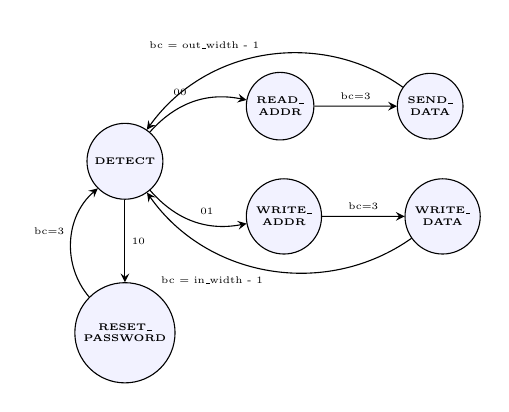
\begin{tikzpicture}[
      scale=0.7, every node/.style={transform shape},
      ->, >=stealth, node distance=1.5cm and 1.5cm,
      state/.style={circle, draw, minimum size=1.1cm, font=\tiny\bfseries, align=center, fill=blue!5},
      transition/.style={font=\tiny, auto}
  ]
      \node[state] (detect) {DETECT};
      \node[state, right=of detect, yshift=1.0cm] (raddr) {READ\_\\ADDR};
      \node[state, right=of raddr] (rdata) {SEND\_\\DATA};
      \node[state, right=of detect, yshift=-1.0cm] (waddr) {WRITE\_\\ADDR};
      \node[state, right=of waddr] (wdata) {WRITE\_\\DATA};
      \node[state, below=of detect] (srst) {RESET\_\\PASSWORD};

      \path (detect) edge[bend left] node[transition] {00} (raddr);
      \path (detect) edge[bend right] node[transition] {01} (waddr);
      \path (detect) edge node[transition] {10} (srst);
      
      \path (raddr) edge node[transition] {bc=3} (rdata);
      \path (rdata) edge[bend right=45] node[transition, swap] {bc = out\_width - 1} (detect);
      
      \path (waddr) edge node[transition] {bc=3} (wdata);
      \path (wdata) edge[bend left=45] node[transition] {bc = in\_width - 1} (detect);
      
      \path (srst) edge[bend left=45] node[transition] {bc=3} (detect);
  \end{tikzpicture}
\end{frame}

% Slide 13: Method 2 Algorithm
\begin{frame}[fragile]{Method 2: ROM Lookup Table Algorithm}
  \begin{block}{Controller ROM Lookup \& Interface Logic}
    \footnotesize
    \begin{algorithmic}[1]
      \STATE Assert $\text{CS} \leftarrow 0$
      \STATE Shift out \texttt{Mode} (2 bits: \texttt{00}=Read, \texttt{01}=Write)
      \STATE Shift out 4-bit sensor address $A$
      \STATE ROM Lookup: 
      \STATE \quad $\text{in\_width}, \text{in\_start} \leftarrow \text{ROM}[A]$
      \STATE \quad $\text{out\_width}, \text{out\_start} \leftarrow \text{ROM}[A]$
      \IF{\texttt{Mode == 01} (Write)}
        \FOR{$i = 0$ \TO $\text{in\_width} - 1$}
          \STATE Shift out payload bit on MOSI
          \STATE $\text{write\_reg}[(\text{in\_start} + i) \pmod{16}] \leftarrow \text{MOSI}$
        \ENDFOR
      \ELSIF{\texttt{Mode == 00} (Read)}
        \FOR{$i = 0$ \TO $\text{out\_width} - 1$}
          \STATE Read MISO bit $\leftarrow \text{read\_reg}[(\text{out\_start} + i) \pmod{16}]$
        \ENDFOR
      \ENDIF
      \STATE Deassert $\text{CS} \leftarrow 1$
    \end{algorithmic}
  \end{block}
\end{frame}

\section{Verilog Implementation}

% Slide 11: ROM Code Listing
\begin{frame}[fragile]{Verilog Code Snippet: slave\_info\_rom}
  \begin{lstlisting}[language=Verilog]
module slave_info_rom (
    input  [3:0] addr,
    output reg [3:0] in_width,
    output reg [3:0] out_width,
    output reg [3:0] in_start,
    output reg [3:0] out_start
);
    always @(*) begin
        case (addr)
            4'd0: begin
                in_width  = 4'd3;   out_width = 4'd4;
                in_start  = 4'd0;   out_start = 4'd0;
            end
            4'd1: begin
                in_width  = 4'd4;   out_width = 4'd4;
                in_start  = 4'd3;   out_start = 4'd5;
            end
            default: begin
                in_width  = 4'd4;   out_width = 4'd4;
                in_start  = 4'd12;  out_start = 4'd12;
            end
        endcase
    end
endmodule
  \end{lstlisting}
\end{frame}

% Slide 12: Code optimizations
\begin{frame}{Verilog Code Optimization Details}
  \begin{itemize}
    \item \textbf{Replacement of Modulo Operators:}
    \begin{itemize}
      \item Modulo division (\texttt{\% 16}) compiles to complex, high-latency division blocks during synthesis.
      \item Optimized to bitwise AND masks (\texttt{\& 4'b1111}) to generate instantaneous 1-cycle logic paths.
    \end{itemize}
    \item \textbf{Single-Driver Assurance:}
    \begin{itemize}
      \item All operations updating the registers are strictly confined to a single synchronous clock block.
      \item Prevents multi-source synthesis errors during compilation.
    \end{itemize}
    \item \textbf{MISO Tri-state Buffering:}
    \begin{itemize}
      \item MISO is explicitly assigned to high-impedance (\texttt{1'bz}) when \texttt{cs} is high.
      \item Allows sharing the physical line on a multi-peripheral bus.
    \end{itemize}
  \end{itemize}
\end{frame}

\section{FPGA \& Web Validation}

% Slide 13: FPGA Implementation
\begin{frame}{FPGA Board Integration}
  \begin{columns}
    \begin{column}{0.5\textwidth}
      \textbf{Validation Environment:}
      \begin{itemize}
        \item Implemented on Xilinx Artix-7 FPGA (\texttt{xc7a35tcsg324-1}) in Vivado.
        \item Emulates real-time sensor inputs using 16 physical DIP switches.
        \item Dynamic driver multiplexes \texttt{read\_reg} (hex) and \texttt{write\_reg} on an 8-digit 7-segment display.
        \item Board status mapped to LEDs.
      \end{itemize}
    \end{column}
    \begin{column}{0.5\textwidth}
      \centering
      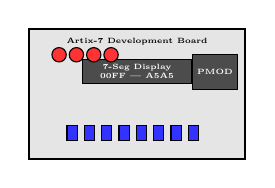
\begin{tikzpicture}[
          scale=0.55, every node/.style={transform shape},
          board/.style={draw, rectangle, minimum height=3.0cm, minimum width=5.0cm, fill=gray!20, thick},
          component/.style={draw, rectangle, minimum height=0.5cm, minimum width=1.0cm, fill=black!70, text=white, font=\tiny\bfseries, align=center},
          led/.style={draw, circle, minimum size=0.15cm, fill=red!80},
          sw/.style={draw, rectangle, minimum height=0.35cm, minimum width=0.12cm, fill=blue!80}
      ]
          \node [board] (pcb) {};
          \node at ($(pcb.north)+(0,-0.3)$) [font=\tiny\bfseries] {Artix-7 Development Board};
          \node [component, minimum width=2.5cm] (seg) at ($(pcb.north)+(0,-1.0)$) {7-Seg Display\\00FF | A5A5};
          \foreach \x in {-1.5,-1.1,...,1.5} {
              \node [sw] at (\x, -0.9) {};
          }
          \foreach \x in {-1.8,-1.4,-1.0,-0.6} {
              \node [led] at (\x, 0.9) {};
          }
          \node [component, minimum height=0.8cm, minimum width=0.6cm] (pmode) at (1.8, 0.5) {PMOD};
      \end{tikzpicture}
    \end{column}
  \end{columns}
\end{frame}

% Slide 14: ESP32 Integration
\begin{frame}{ESP32 Web Server Integration}
  \begin{itemize}
    \item \textbf{Remote Monitoring Architecture:}
    \begin{itemize}
      \item ESP32 micro-controller hosts a local web server (HTTP / WebSockets).
      \item Provides interactive controls (Select Sensor, Write hex payload, triggering Read/Write operations).
      \item ESP32 drives the FPGA pins through physical PMOD SPI headers.
    \end{itemize}
  \end{itemize}
  \vspace{0.2cm}
  \centering
  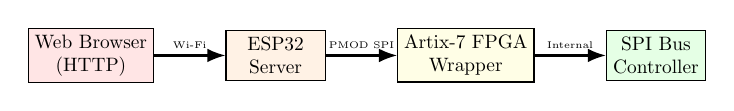
\begin{tikzpicture}[
      scale=0.7, every node/.style={transform shape},
      box/.style={draw, rectangle, minimum height=0.8cm, minimum width=1.8cm, align=center, fill=blue!5},
      arrow/.style={draw, -{Latex[scale=1.0]}, thick}
  ]
      \node [box, fill=red!10] (web) {Web Browser\\(HTTP)};
      \node [box, right=of web, fill=orange!10, xshift=0.3cm] (esp) {ESP32\\Server};
      \node [box, right=of esp, fill=yellow!10, xshift=0.3cm] (fpga) {Artix-7 FPGA\\Wrapper};
      \node [box, right=of fpga, fill=green!10, xshift=0.3cm] (bus) {SPI Bus\\Controller};

      \path [arrow] (web) -- node[above, font=\tiny] {Wi-Fi} (esp);
      \path [arrow] (esp) -- node[above, font=\tiny] {PMOD SPI} (fpga);
      \path [arrow] (fpga) -- node[above, font=\tiny] {Internal} (bus);
  \end{tikzpicture}
\end{frame}

\section{Experimental Results}

% Slide 15: Resource comparison
\begin{frame}{Resource Utilization Results}
  \begin{table}
    \centering\small
    \begin{tabular}{lccc}
      \toprule
      \textbf{FPGA Resource} & \textbf{Method 1} & \textbf{Method 2} & \textbf{Available (Artix-7)} \\
      \midrule
      LUTs & 78 & 62 & 20,800 \\
      Flip-Flops & 68 & 54 & 41,600 \\
      BRAM Blocks & 0 & 0 & 50 \\
      Setup Slack & $+15.24\text{ ns}$ & $+15.24\text{ ns}$ & Target: 50 MHz \\
      Max Frequency ($F_{\text{max}}$) & $142.8\text{ MHz}$ & $166.4\text{ MHz}$ & — \\
      \bottomrule
    \end{tabular}
    \caption{Resource and Timing Analysis Report}
  \end{table}
  \begin{itemize}
    \item \textbf{ROM Lookup Efficiency:} Method 2 shows a \textbf{20.5\% reduction in LUT usage} and a \textbf{20.6\% reduction in Flip-Flops} due to a smaller FSM (6 vs 9 states).
  \end{itemize}
\end{frame}

% Slide 16: Detailed comparison
\begin{frame}{Methodology Comparison Matrix}
  \begin{table}
    \centering\tiny
    \begin{tabular}{lll}
      \toprule
      \textbf{Metric} & \textbf{Method 1: Address + Length} & \textbf{Method 2: ROM Lookup} \\
      \midrule
      Packet Size (Write 8b) & 19 bits & 14 bits \\
      Control Overhead & 11 bits (57.8\% of packet) & 6 bits (42.8\% of packet) \\
      Latency (Write 4b) & 15 cycles ($1.50\ \mu\text{s}$ at 10 MHz) & 10 cycles ($1.00\ \mu\text{s}$ at 10 MHz) \\
      On-Chip Memory (ROM) & Zero & 80 bits \\
      Flexibility & High (software-defined) & Static (requires bitstream rebuild) \\
      Continuous Throughput & Moderate ($5.26\text{ Mbps}$) & High ($7.14\text{ Mbps}$) \\
      Recommended for & Software prototyping, dynamic nodes & Production systems, fixed devices \\
      \bottomrule
    \end{tabular}
    \caption{Detailed Comparison of Implemented SPI Methods}
  \end{table}
  \begin{itemize}
    \item \textbf{Latency Reduction:} Method 2 provides a \textbf{33.3\% improvement in transaction speed} by removing the length configuration phase.
  \end{itemize}
\end{frame}

% Slide 19: Pros and Cons Comparison
\begin{frame}{Methodology Comparison: Pros and Cons}
  \begin{table}
    \centering\tiny
    \begin{tabular}{lp{4.2cm}p{4.2cm}}
      \toprule
      \textbf{Method} & \textbf{Advantages (Pros)} & \textbf{Drawbacks (Cons)} \\
      \midrule
      \textbf{Method 1: Address + Length} & 
        - Software-defined dynamic widths \newline
        - No re-synthesis required for new sensors \newline
        - High runtime flexibility & 
        - Large control overhead (11 bits per write) \newline
        - Higher transaction latency \newline
        - Complex state machine \\
      \midrule
      \textbf{Method 2: ROM Lookup} & 
        - Very low control overhead (6 bits) \newline
        - 33.3\% faster data transfers \newline
        - 20\% smaller FPGA logical footprint & 
        - Hardcoded register metadata \newline
        - Changing specs requires FPGA re-synthesis \newline
        - Constrained by ROM space \\
      \bottomrule
    \end{tabular}
    \caption{Pros and Cons Tradeoffs}
  \end{table}
\end{frame}

\section{Conclusion \& Future Work}

% Slide 17: Conclusion
\begin{frame}{Conclusion \& Future Work}
  \begin{itemize}
    \item \textbf{Key Accomplishments:}
    \begin{itemize}
      \item Successfully resolved the $O(N)$ routing footprint of standard SPI configurations.
      \item Decoupled master clock phase dependencies from sensor domains using an asynchronous CDC FIFO interface.
      \item Method 2 (ROM Lookup) proved to be 33.3\% faster and consumed 20.5\% less logic gates compared to Method 1.
    \end{itemize}
    \item \textbf{Future Directions:}
    \begin{itemize}
      \item \textbf{Programmable RAM Configuration Map:} Allow boot-time updates to sensor offsets, giving Method 2 the dynamic capability of Method 1.
      \item \textbf{DMA Interface:} Integrate Direct Memory Access to write data blocks directly to memory, avoiding CPU cycle consumption.
      \item \textbf{Bus Protocol Wrappers:} Expose standard AMBA AXI4-Lite or Wishbone wrappers for easy SoC system integration.
    \end{itemize}
  \end{itemize}
\end{frame}

\end{document}
